\subsection{Deblending \footnote{This section assumes that a dection section has already been written. Some changes might be necessary if there are topics not covered in the detection section or topics that are duplicated in this section."}}

\label{sec:deblending}

Deblending in the science pipelines is performed differently for single-band (visit) image processing vs. multi-band (coadd) image processing.
This section gives a basic description of each algorithm.

\subsubsection{Single-band Deblending}

\label{sec:singleband_deblending}

Deblending on single-band images (ie. visit) is performed using the \texttt{meas\_deblender} package and is based on the deblender used in SDSS (citation needed), with a few differences that will be discussed shortly.
Similar to the SDSS deblender, the LSST deblender creates a template for each source in a blend using a very simple (yet computationally efficient) model for each peak position in a parent Footprint.
Once a template has been created for each peak in the blend, the deblender combines all of the source templates into a single blend model by summing their values in each pixel.
For each pixel in a source template, the ratio of the source template value to the total blend model is calculated and used to weight the pixel value from the image to create a model for each source.
The source models are thus flux conserving in that adding them together will yield the original image except for pixels that do not appear in any of the individual templates.
A cleanup algorithm is then run to allocate the remaining pixels to one of the sources in the blend based on a set of criteria including distance to the center, brighness of the nearest sources, etc.

\subsubsection{Deblender Template Generation}

The main ansatz of the SDSS deblending algorithm is that the flux from stars and galaxies in a ground based telescope is nearly 180 degree symmetric.
Figure \ref{fig:simple_blend} illustrates how a 1D slice through the center of two blended sources can exploit this symmetry by setting the pixels on opposite sides of the (integer) center pixel to the minimum value of both pixels.
In other words, for simple blends of only two sources the deblender can use the flux on the non-blended side to constrain the value of the flux on the blended side.
Despite the fact that stars (PSFs) and galaxies are not exactly symmetric, especially since their position is not exactly centered in the center of a single pixel, this algorithm works quite well for generating templates in simple blends that very nearly approximate each source when redistributing flux from the image.

For sources with low SNR the algorithm fails due to noise in the image, generating galaxy templates that are typically very jagged and unphysical.
To combat this, for each \texttt{peak} in the parent \texttt{Footprint} the deblender first attempts to fit the flux from the image with a simple PSF model that allows its position, amplitude, and a linear background, to vary.
If the fit has a reasonable $\chi^2$ value then the deblender will use this scaled PSF model as a template for the source.
Only for sources that cannot be adequately modeled with the PSF are the symmetric templates used.

The main failure point of this algorithm is when three (or more) sources lie along the same axis.
For example, Figure \ref{fig:complex_blend} illustrates a 1D slice through the center of three aligned sources.
In this case the minimum pixel on each side of the central source cannot constrain the flux at that radial location and results in a template that has extra bumps from its neighbors.
This turns out to be more catastrophic than one might expect.
Notice that even the neighboring sources, which have very good templates created by using symmetry on their unblended side, have their resulting models contaminated due to the central object that steals flux from both of them.
In single visits the number of "three in a row" blends is small enough that we sacrifice the quality of the models for efficiency and still use the single-band deblender.
For LSST-depth coadds this becomes a significant problem, as deep coadds can have as much as 40\% of blends having 3 or more sources and a more sophisticated algorithm is needed.

\begin{figure}[htb]
    \centering
    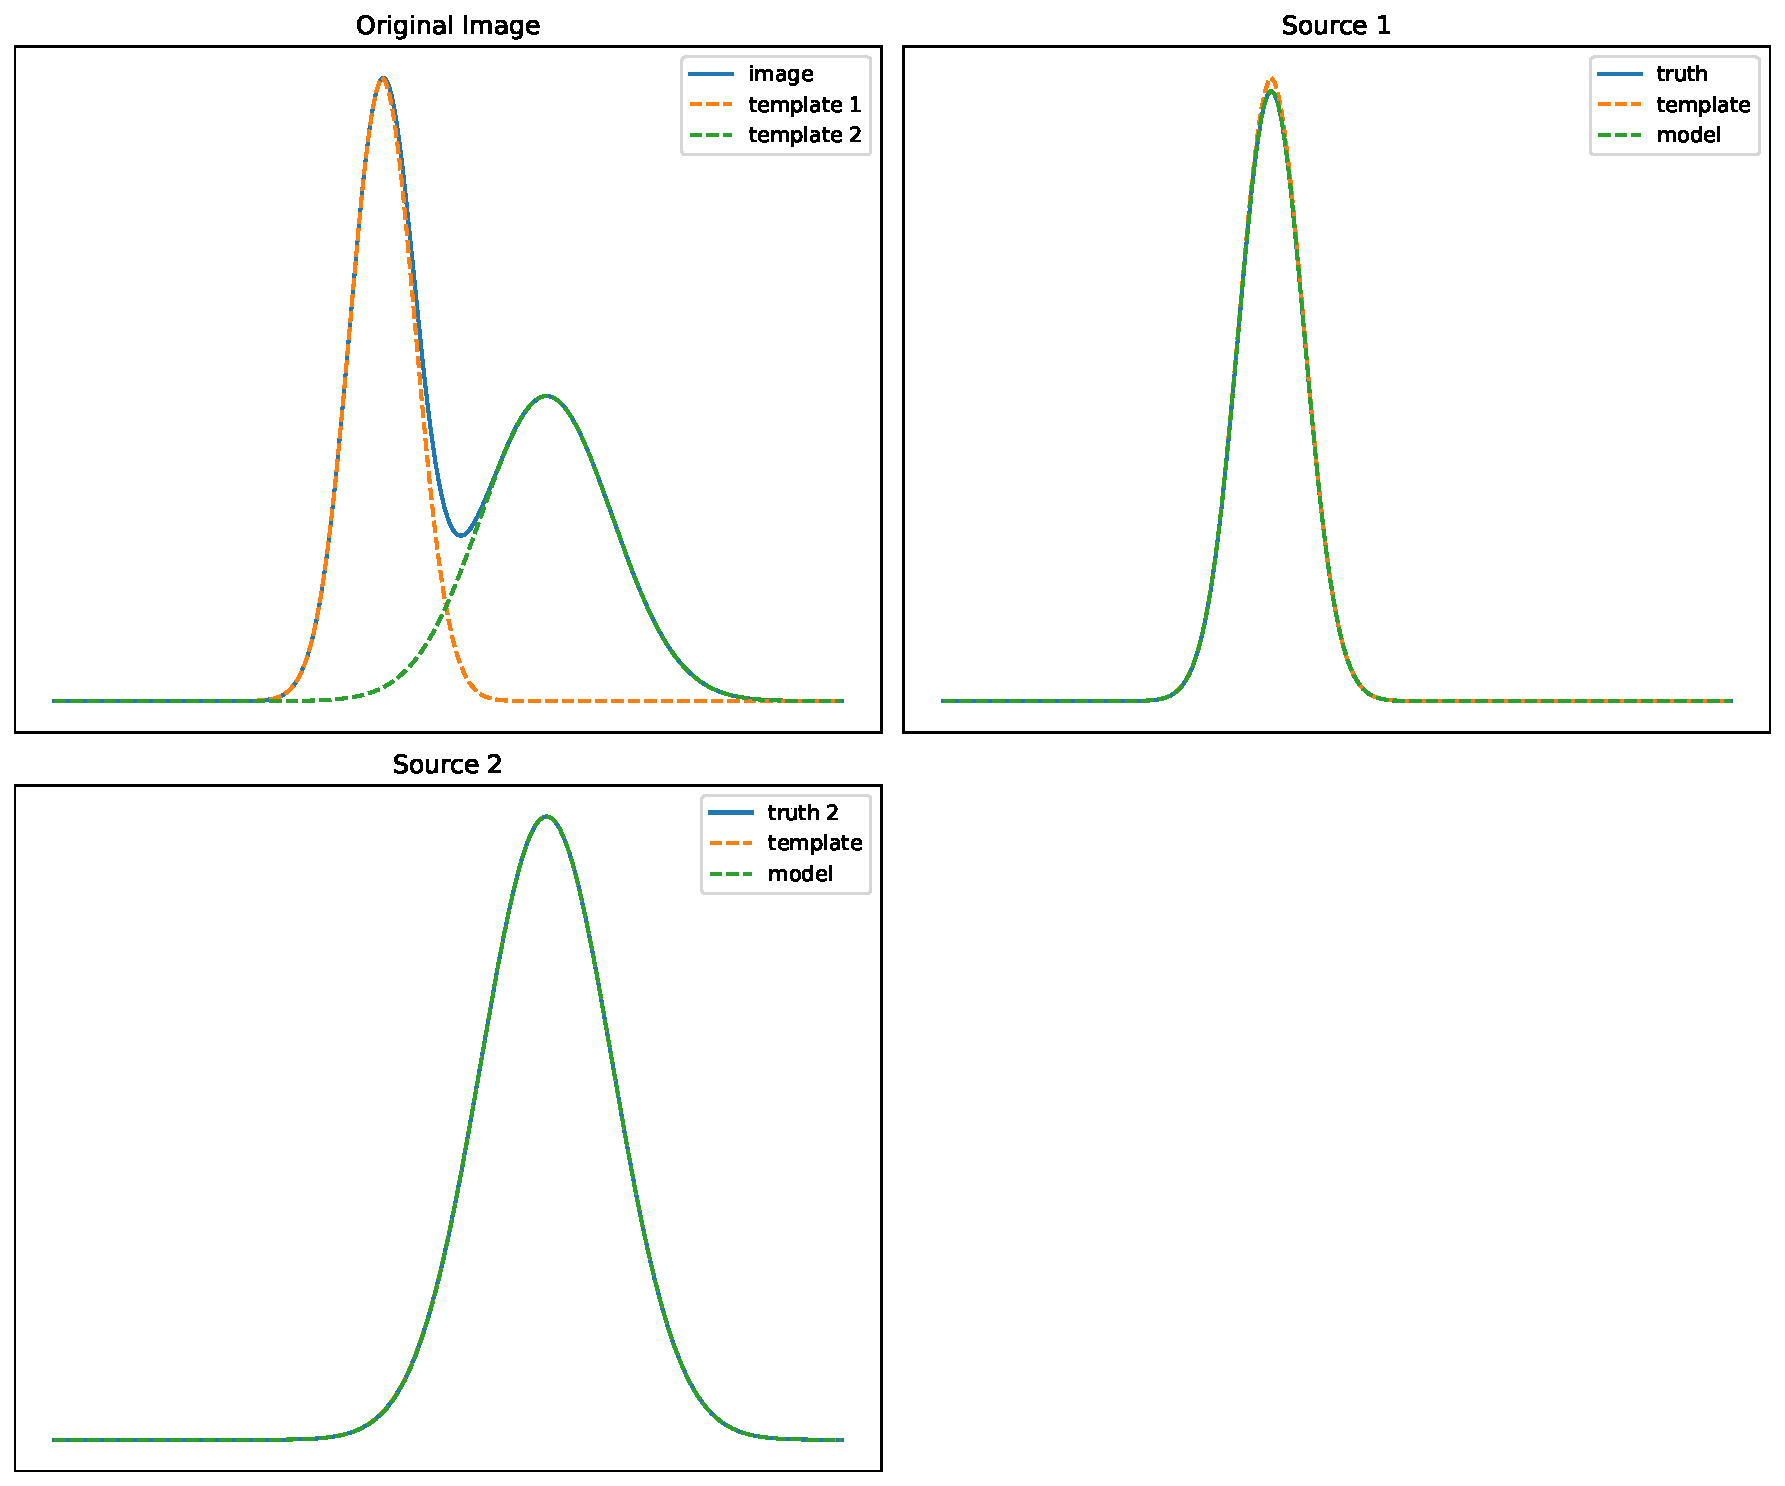
\includegraphics[width=0.48\textwidth]{simple_1D_blend.pdf}
    \caption{A 1D slice of two blended Gaussian sources illustrating how symmetry can be utilized to model blended sources.}
    \label{fig:simple_blend}
\end{figure}

\begin{figure}[htb]
    \centering
    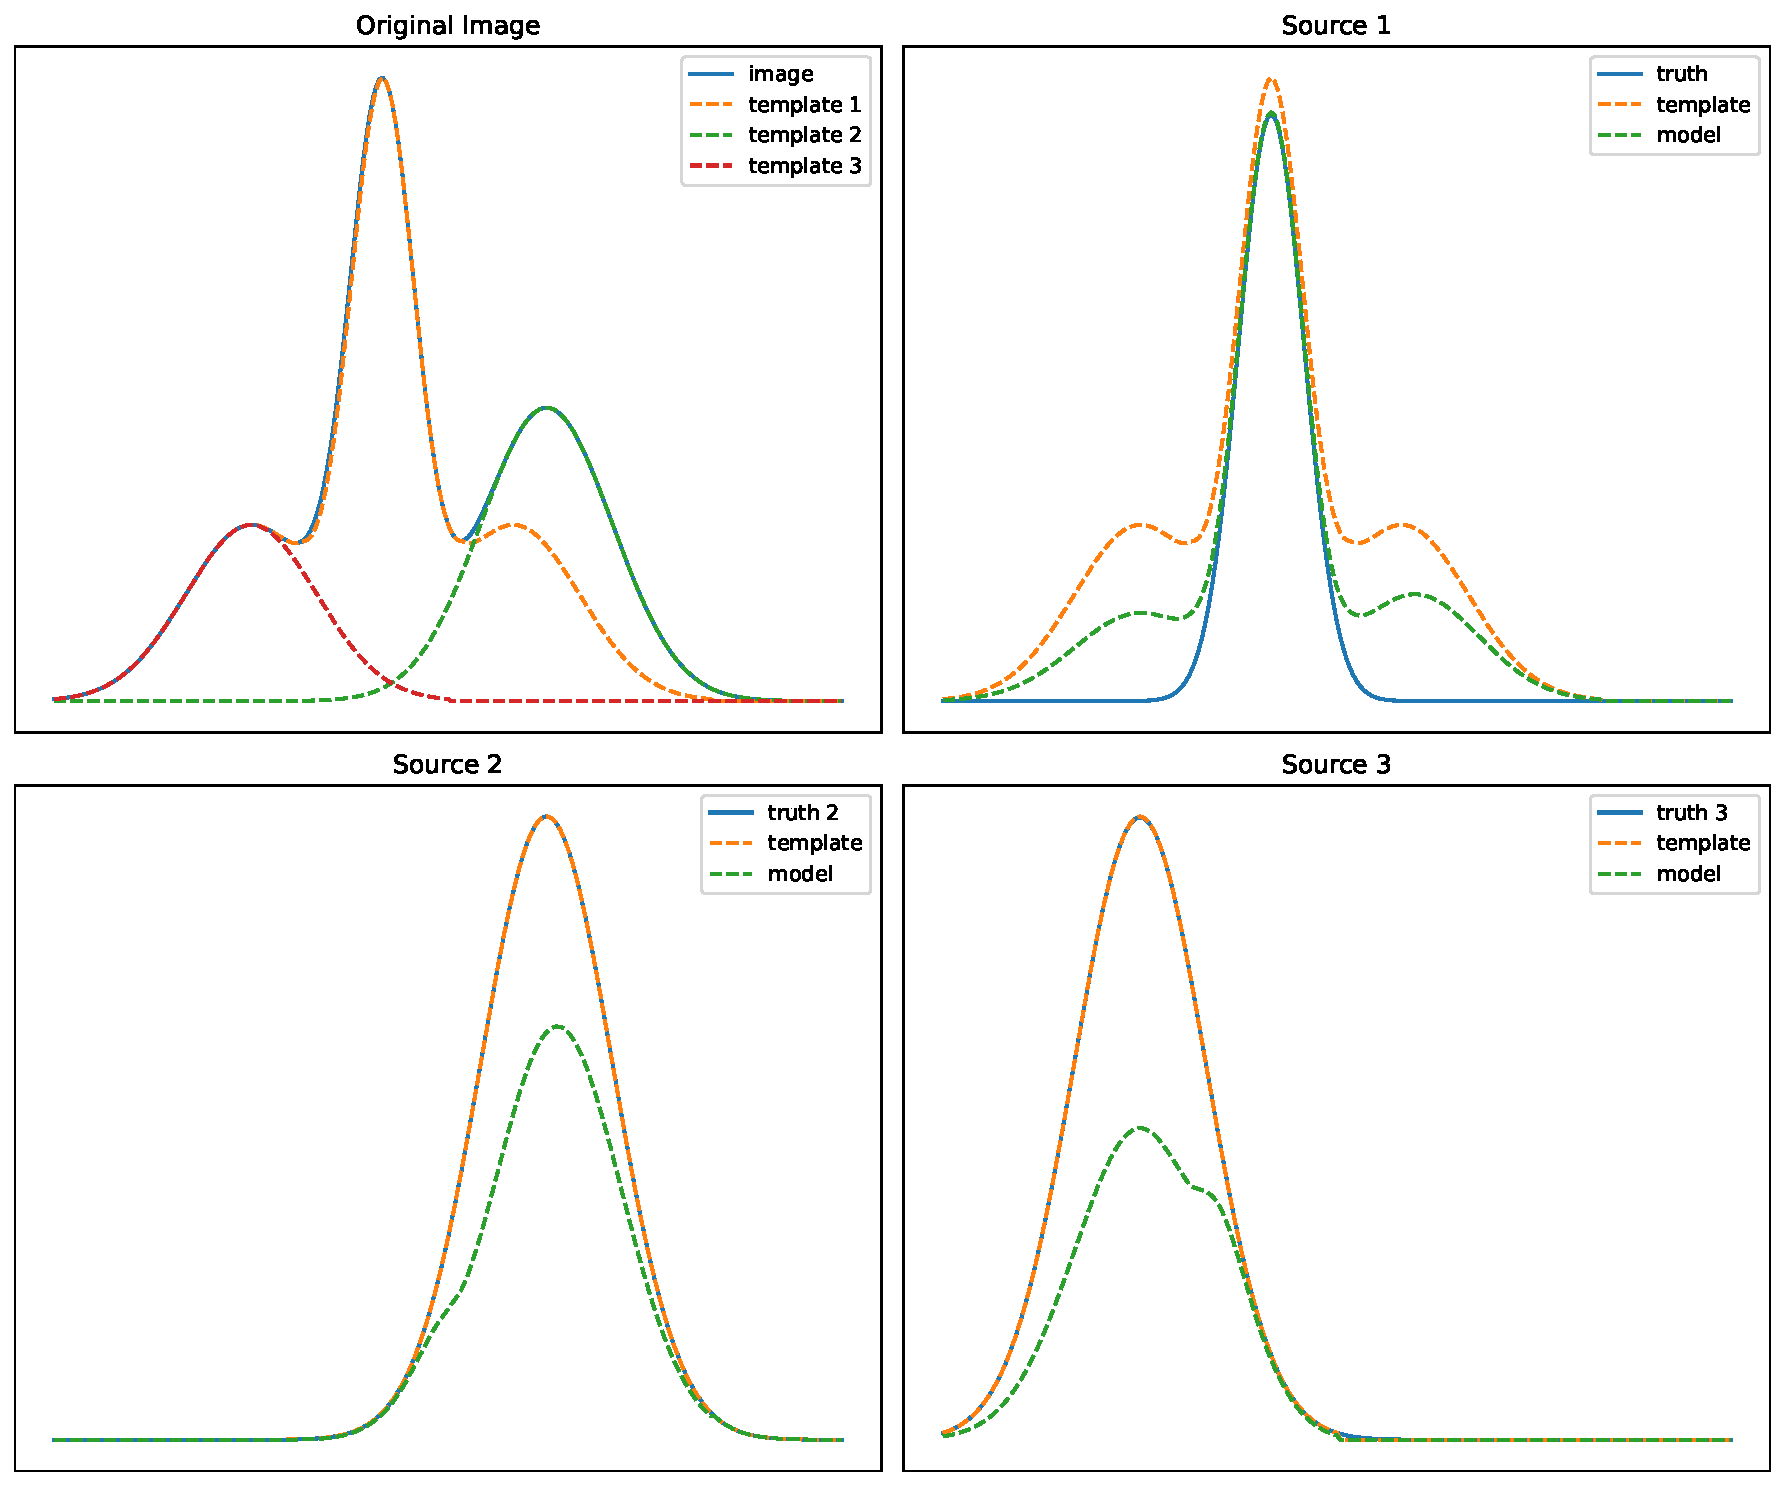
\includegraphics[width=0.48\textwidth]{complex_1D_blend.pdf}
    \caption{A 1D slice through three aligned Gaussian sources, demonstrating a failure case of relying on symmetry for generating deblender templates. Notice that for sources 2 and 3 the templates are reasonable but due to the inability of source 1 to use symmetry to constrain flux in the blended region, the resulting models for all three sources are poor. This catastrophic "three in a row" problem was part of the motivation for creating \texttt{scarlet} to incorporate spectral information and a more rigorous iterative deblending algorithm.}
    \label{fig:complex_blend}
\end{figure}

\subsubsection{Multi-band Deblending}
\label{sec:multiband_deblending}

The multi-band deblender is an implementation of the scarlet deblending algorithm described in \citet{2018A&C....24..129M}.
In our implementation, \texttt{scarlet\_lite}, we have made our own set of simplifying assumptions that are different from the original scarlet algorithm to make it more efficient when used in a large ground based survey like LSST.
Similar to the original \texttt{scarlet} we make the assumption that astrophysical objects can be thought of as a collection of components, where each component has the properties
\begin{itemize}
    \item Components have a single color (spectrum) that is the same in all pixels over its shape (morphology)
    \item Components have flux that monotonically decreases from the center
    \item Component flux is additive
\end{itemize}

The classic example is decomposing a single galaxy into bulge and disk components, where both the bulge and disk share a common center but have different spectra and morphologies.
Something more complex, like a grand design spiral, could in theory be modeled as a source with multiple components, where spiral arms and star forming regions could still be thought of as separate monotonic components.
For the science pipelines we ignore those more complicated structures, as detection typically already shreds large galaxies into multiple sources.
Instead we use a signal to noise cut where low flux sources are modeled with a single component and higher flux sources are modeled with two components.

Scarlet lite initializes models with nearly the same templates as those generated by the single-band deblender.
Using a $\chi^2$-like monochromatic image created by weighting each band by its inverse variance, scarlet lite creates initial morphology models that are symmetric from the center in the monochromatic image, with the additional constraint that the flux is monotonically decreasing from the center.
In order to satisfy the constraint that all pixels in the morphology have the same spectrum, scarlet models exist in a partially deconvolved frame with the seeing of a well sampled but narrow Gaussian.
The initial spectrum of each source is determined using a least squares fit of each monochromatic morphology, convolved with the difference kernel in each band to match the image, for each component.
It then uses proximal-ADAM \citep[PADAM,][]{2019arXiv191010094M} to iteratively update the spectrum and morphology with the given constraints until convergence or a maximum number of iterations is reached.
It should be noted that although we do use symmetry to initialize the scarlet models, we do not implement a symmetry constraint and the final models are not guaranteed to be symmetric.
The models are stored as the \texttt{deepCoadd\_scarletModelData} data product, which contains all of the blends for a single patch.
Like the single-band deblender, the \texttt{scarlet\_lite} models are only used as templates to redistribute flux from the image and all measurements are performed on the flux redistributed models.
